\section{Aim of Study}
The data contains a time-series of the number of sales for 3049 products across 10 different stores, for a total of 30490 items. 
We aim to create several models and compare their performance on predicting the number of sales for all 30490 items for the next 28 days. 
Specifically, we aim to compare the performance of deep learning and machine learning methods.
For deep learning methods, we will compare the performance of Recurrent Neural Networks (RNN) with Artificial Neural Networks (ANN). 
Specifically, the recurrent neural network will be a Long Short-Term Memory (LSTM) model, and the artificial neural network will be a Multi-Layer Perceptron (MLP) model.
Moreover, the machine learning method was chosen to be a LightGBM (LGBM) model. 
Additionally, we will create a hybrid model, consisting of the LSTM model and the best performing model between the MLP and LGBM models, and check if it is able to improve the performance compared to the singular models.


\section{Selection of the Response Variable}
All models will be trained using the Root Mean Square Error (RMSE) as the loss function.
Moreover, the RMSE on the validation set will be used to optimize the hyperparameters of each model.
On the other hand, in order to evaluate and compare the performances of the models, we will obtain the Root Mean Square Scaled Error (RMSSE) of the models on the test set.
Compared to RMSE, RMSSE has the advantage of being scale independent, and so it can be used to compare the accuracy of forecasts across time-series with different scales.
For example, an absolute error of 10 when approximating 100 should have a much higher forecast error than an absolute error of 10 when approximating 1,000,000.
RMSSE is derived from the Mean Absolute Scaled Error (MASE), which is a common measure of accuracy for forecasting problems.
In order to scale the error, the Mean Squared Error (MSE) of the model is compared to the MSE of a naive model, which predicts the sales at each time-step to be the same as the previous time-step.
The original RMSSE uses the in-sample data (training set) for the naive model, since the out of sample data (test set) may not contain enough points to obtain a naive prediction when the forecasting horizon is too short: \cite{yardstick, m5}
\[RMSSE = \sqrt{\frac{MSE_{\,test, \,model}}{MSE_{\,train, \,naive}}}\]
However, since in our study we have a forecasting horizon of 28, we do not have to worry about this issue and hence for simplicity, we will use the out of sample data to obtain the MSE of the naive model:
\[RMSSE = \sqrt{\frac{MSE_{\,test, \,model}}{MSE_{\,test, \,naive}}}\]

Another advantage of RMSSE compared to RMSE is its interpretability. 
The value of RMSSE represents how well a model performs compared to a naive model. 
An \(RMSSE > 1\) means that the model performs worse than the naive model and should be discarded, an \(RMSSE = 1\) means the model performs just as well as the naive model, and an \(RMSSE < 1\) means the model performs better than the naive model. 
The closer the value of RMSSE is to 0, the better the model performs.

In addition to RMSSE, the Mean Error (ME) of the models will be obtained in order to see whether the models have a tendency to over-forecast or under-forecast the target sale values.

\section{Choice of Factors and Levels}
The following four models will be evaluated and compared in this project.

\begin{enumerate}
  \item LSTM,
  \item Artificial Neural Network,
  \item LightGBM, and
  \item Hybrid.
\end{enumerate}

The hyperparameters of all models will be optimized using Bayesian Optimization over a given range of hyperparameter values.
In Bayesian optimization, the optimizer starts with a prior belief of the environment and with every combination of hyperparameter values that it examines, it updates its belief of the environment and looks for the hyperparameter values that will maximize the chance of improving our performance in the next round. 
For the LSTM and MLP models, Bayesian optimization was used to optimize the number of hidden layers, number of hidden units, learning rate, learning rate decay, dropout rate, and batch size.
Moreover, Bayesian optimization was used to decide whether a batch normalization layer should be included in the architecture of the models. 
Additionally, the number of historical observations for the LSTM model was optimized as well.
On the other hand, the LGBM model has many hyperparameters that can be optimized. 
In this project, Bayesian optimization was used to find the best hyperparameter values for the learning rate, the fraction of the features used, the value of lambda for L2 regularization, the minimum data in each leaf, and the number of leaves for the model.

\section{Choice of Experimental Design}
The time-series include a total of 1941 days of sales data, which will be split into training, validation, and test sets. 
The training set will include 1885 days of time-series data, which will be used to train the hybrid model.
The validation set will include a time-series data for the next 28 days, from day 1886 to day 1913, which will be used for hyperparameter optimization.
Finally, the test set will include the last 28 days of time-series data, from day 1914 to day 1941, which will be used to evaluate and compare the models and assess their generalization on unseen data. 

Since the dataset contains the sales data for 3049 products sold across ten different stores, we are dealing with a multi-channel problem. 
It is important to take into account the effects of aggregate demand on the sales, as well as the effects of one item on the sales of another item.
Hence, rather than training separate models for each item, a single model will be created for all items.
Furthermore, since we want to forecast the daily sales for the next 28 days, we are dealing with a multi-step forecasting problem. 
There are three main methods for dealing with multi-step forecasting problems.
In the first method, a separate model is trained for each step. 
However, this is not very practical, not only because of the number of models that will need to be trained, but also because normally the sales on each day are somehow dependent on the sales of the previous days, which is not considered in this method.
In the second method, a single model predicts all steps at once.
However, this method also lacks the ability to obtain any information from the previous steps of the forecasting horizon to predict future steps.
Alternatively, one can use a single model to forecast each step one at a time, where at each step, the previous forecasted values are used to forecast the sales of the current day.
This method can be more consistent as it takes into account the effects of previous days when forecasting many days ahead.
Hence, this is the method that will be used in this project to deal with multi-step forecasting.

In the rest of this section, we will talk about the two experiments that will be performed in this project.

\subsection*{Experiment 1}
Three singular models (LSTM, MLP, and LGBM) will be constructed, and their performances will be evaluated and compared for 28-days ahead point forecasts. 
In order to help the MLP and LGBM models learn the seasonality from the time-series data and look more than one step in the past, we will introduce lag features in the dataset. 
To produce lag features, we will shift the sales data to the future by a fixed number of days. 
For example, the lag 7 of the sales at time-step \(t\) for an item will be its sales value at time-step \(t-7\). 
In addition to the lag features, we will introduce rolling means and rolling standard deviations of the sales with various sliding-window sizes in order to help the models learn from the time-series data.

\subsection*{Experiment 2}
\begin{wrapfigure}[11]{r}{0.45\textwidth}
    \vspace{-8.5mm}
    \fbox{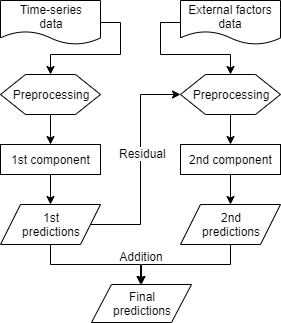
\includegraphics[width=0.43\textwidth]{figures/results/hyb_summary.PNG}}
    \captionof{figure}{Structure of the hybrid model.}
    \label{fig:hyb_summary}
\end{wrapfigure}
For the second experiment, a hybrid model will be constructed and its performance will be compared with the performances of its two components.
There are two elements in the dataset that must be considered when constructing the model's architecture.
The first element is the time-series data and the second element is all other data, such as promotions and holidays, that are considered to be external factors and might have an influence on the time-series data.
Hence, the first component of the hybrid model will be the LSTM network that will learn from the time-series data. 
LSTM networks are able to handle both the linear and nonlinear demand variations, which eliminates the need of multiple methods for different demand variations \cite{c8}.
The second component of the hybrid model will serve to learn from the external factors. 
Specifically, the second component will predict the difference in LSTM's predictions and actual demand based on the external factors.
To elaborate, assume we want to predict the demand for a time period, \(t \geq 1\), with the actual demand data, \(Y_t\), known. 
If the LSTM model makes predictions, \(\hat{y_t}\), for this time period, then the difference in the LSTM's predictions and the actual demand is calculated as:
\[\Delta y_t = Y_t - \hat{y_t} \vspace{-2mm}\]
This difference, \(\Delta y_t\) will be used as the independent variable(s) in the second component of the hybrid model, along with the external factors as the dependant variables. The second component will then be trained to predict this difference, \(\Delta \hat{y_t}\), based on the external factors. At last, the final forecast, \(\hat{Y_t}\), will be obtained by aggregating the predictions of the two model components \cite{c8}:
\vspace{-5mm}
\[\hat{Y_t} = \hat{y_t} + \Delta \hat{y_t} \vspace{-5mm}\]
The study done in \cite{c8} has already used a Random Forest (RF) network as the second component for forecasting demands of a multi-channel retail, and they were able to achieve very accurate predictions.
In this study, we will use the best performing model between MLP and LGBM as the second component of the hybrid model. 
Similar to random forest, LGBM is a tree-based learning model, however, LGBM uses gradient boosting to enhance the performance of the model, whereas random forest uses bagging.

\section{Technologies}
All models will be created using \texttt{Python}. 
The LSTM and ANN models will be constructed using the package \texttt{keras} and LGBM will be implemented using the package \texttt{lightgbm}. 
The Bayesian optimization will be created using the \texttt{bayesian-optimization} package.
Moreover, other packages, such as \texttt{pandas} and \texttt{scikit-learn}, will be used for data preprocessing and model evaluation.